\documentclass[12pt,aspectratio=169]{beamer}
\usecolortheme{udec}
\usetheme{udec}
\usepackage{graphicx}
\graphicspath{{img/},{slides/}}
\usepackage{pgffor}
\usepackage{tikz}
\usepackage{fontspec}
\usepackage{gelasio}
\usefonttheme{serif}
\setmainfont{Gelasio}
\usepackage{polyglossia}
\setmainlanguage{spanish}
% \setbeameroption{show notes on second screen=bottom}

\newcommand<>{\fullsizegraphic}[1]{
	\begin{tikzpicture}[remember picture,overlay]
	\node[at=(current page.center)] {
		\includegraphics{#1}
	};
	\end{tikzpicture}
}

\usepackage{listings}
\usepackage{xcolor}
\definecolor{codegreen}{rgb}{0,0.6,0}
\definecolor{codegray}{rgb}{0.5,0.5,0.5}
\definecolor{codepurple}{rgb}{0.58,0,0.82}
\definecolor{backcolour}{rgb}{0.95,0.95,0.92}
\lstdefinestyle{mystyle}{
    backgroundcolor=\color{backcolour},   
    commentstyle=\color{codegreen},
    keywordstyle=\color{magenta},
    numberstyle=\tiny\color{codegray},
    stringstyle=\color{codepurple},
    basicstyle=\ttfamily\footnotesize,
    breakatwhitespace=false,         
    breaklines=true,                 
    captionpos=b,                    
    keepspaces=true,                 
    numbers=left,                    
    numbersep=5pt,                  
    showspaces=false,                
    showstringspaces=false,
    showtabs=false,                  
    tabsize=2
}
\lstset{style=mystyle}
\usepackage{dirtytalk}

\title{Establecimiento de protocolo de comunicación entre X-Plane y microcontroladores externos}
\subtitle{Proyecto de ingeniería aeroespacial}
\author{Por Germán Quijada}
\institute{Profesor guía:\\Bernardo Hernández}

\begin{document}
\begin{frame}[noframenumbering]
\maketitle
\end{frame}

\begin{frame}{Contenidos}
\tableofcontents
\end{frame}

%% Introducción
\section{Concepto}

\begin{frame}{Concepto}
En el simulador de vuelo del laboratorio de técnicas aeroespaciales, establecer un \emph{protocolo de comunicación} entre el software de simulación \emph{X-Plane} y \emph{microcontroladores externos}.
\note{
En el simulador de vuelo del laboratorio de técnicas aeroespaciales, establecer un protocolo de comunicación entre el software de simulación X-Plane y microcontroladores externos

Se define que en el laboratorio de técnicas aeroespaciales de la universidad de Concepción solo para acotar el problema, pero en la práctica no hay razón para que lo implementado en el laboratorio no funcione en otro computador personal
}
\end{frame}

\subsection{Actores en la comunicación}
\begin{frame}[noframenumbering]
\subsectionpage
\note{
Analicemos un poco el problema desde lo más básico, que es X-Plane y que es un microcontrolador y por qué se querría establecer comunicación entre ellos
}
\end{frame}

\begin{frame}{X-Plane}
\begin{itemize}
	\item Software de simulación de vuelo
	\item<2-> Utilizado en entornos de entrenamiento certificados\footnotemark
	\item<3-> Herramienta ingenieril\footnotemark
	\item<4-> Funcionalidad agregada con plug-ins
	\item<5-> Interfaz de comunicación UDP
\end{itemize}
\only<2->{
	\footnotetext[1]<2->{\url{https://x-plane.helpscoutdocs.com/article/31-faa-certification}}
	\footnotetext[2]<3->{\url{https://www.x-plane.com/desktop/meet\_x-plane}}
}
\note<1>{
	X-Plane es un simulador de vuelo que destaca por sus físicas de vuelo realistas y es popular tanto para entusiastas de la aviación como para pilotos en entrenamiento.
}
\note<2>{
	En conjunto con el hardware apropiado, X-Plane cumple con los requisitos y normas de simulación de vuelo necesarios para su uso en entrenamiento de pilotos y otras aplicaciones relacionadas con la aviación.
}
\note<3>{
	Debido a lo realista del modelo de vuelo, X-Plane puede evaluar el rendimiento de nuevas configuraciones de aeronaves, realizar análisis de vuelo, simular condiciones específicas y validar conceptos antes de la construcción física.
}
\note<4>{
	X-Plane cuenta con herramientas de desarrollo para crear plug-ins personalizados y en internet hay muchos publicados por terceros, esta podría ser una forma de abordar la implementación del protocolo.
}
\note<5>{
	Otra forma de establecer comunicación es por medio de la interfaz UDP integrada en el simulador, sin embargo este medio está orientado a desarrolladores y no es fácil de usar.
}
\end{frame}

\begin{frame}
\centering
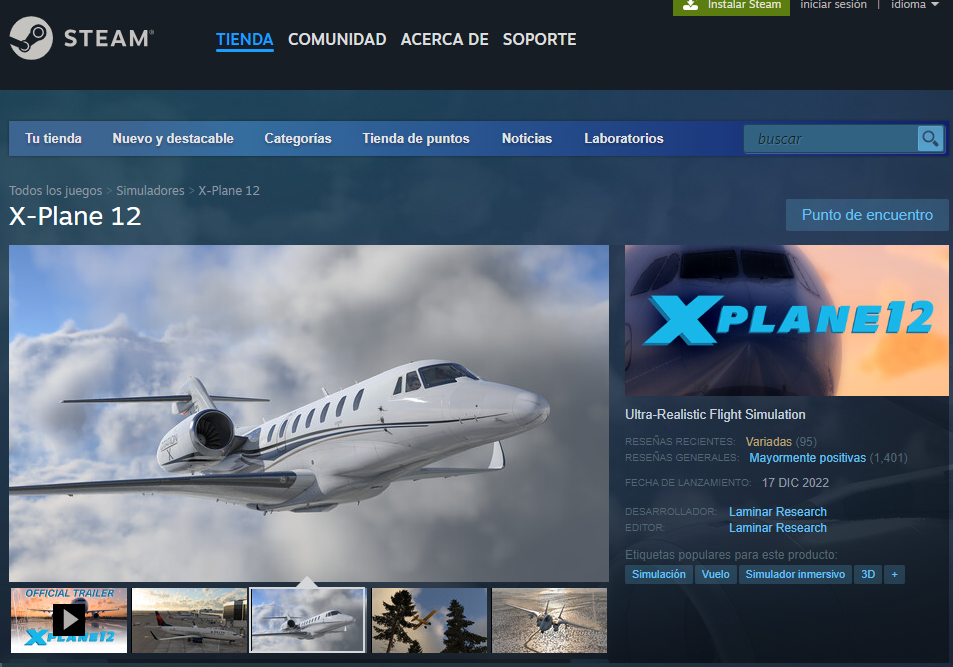
\includegraphics[width=0.8\textwidth]{xplane-steam.png}
\footnotemark
\footnotetext{\url{https://store.steampowered.com/app/2014780/XPlane_12/}}
\end{frame}

\begin{frame}{Microcontroladores}
\begin{itemize}
	\item Pequeños dispositivos electrónicos integrados
	\item<2-> Especializados
	\item<3-> Interfaces estandarizadas ($I^2C$, Serial, UART)
	\item<4-> Bajo costo
\end{itemize}
\note<1>{
	El microcontrolador es un dispositivo electrónico integrado que en sus formas más simples combina una unidad de procesamiento, memoria y alguna interfaz de entrada y salida de señales. Se podría decir que es como un computador, pero muy muy pequeño y utilizados para una sola tarea especifica.
}
\note<2>{
	Una vez programado se tiene mucha seguridad que en cada encendido el microcontrolador ejecutara las órdenes tal cual fueron escritas y nada más. Sin los problemas que podría ocasionar el tener un sistema operativo completo.
}
\note<3>{
	Por lo general los microcontroladores habilitan una o más interfaces de comunicación con otros microcontroladores o cualquier dispositivo que implemente la misma interfaz. Algunos ejemplos son I2C, Serial y UART entre muchos otros.
}
\note<4>{
	Y por lo último los microcontroladores al no presentar funciones más complejas pueden llegar a ser muy baratos sin necesidad de comprometer alguna funcionalidad. En la práctica la condicional para elegir entre un microcontrolador u otro va a ser las funciones de cada uno en vez del precio. 
}
\end{frame}

\begin{frame}
\begin{columns}
\begin{column}{0.45\textwidth}{
	\begin{figure}[t]
		\centering
		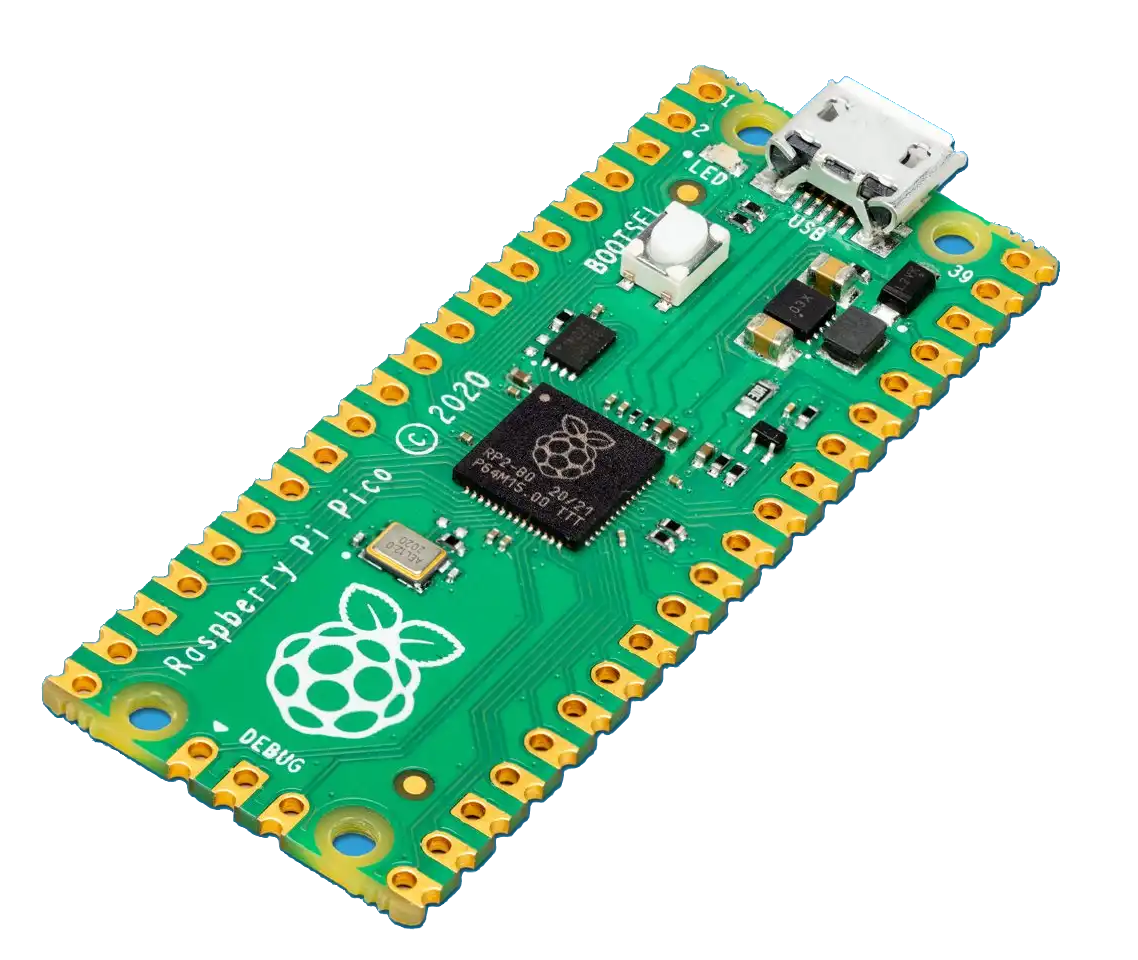
\includegraphics[width=0.6\textwidth]{raspberry-pi-pico.png}
		\caption{Raspberry Pi Pico\footnotemark}
\end{figure}
}
\end{column}
\begin{column}{0.45\textwidth}{
	\begin{figure}[t]
		\centering
		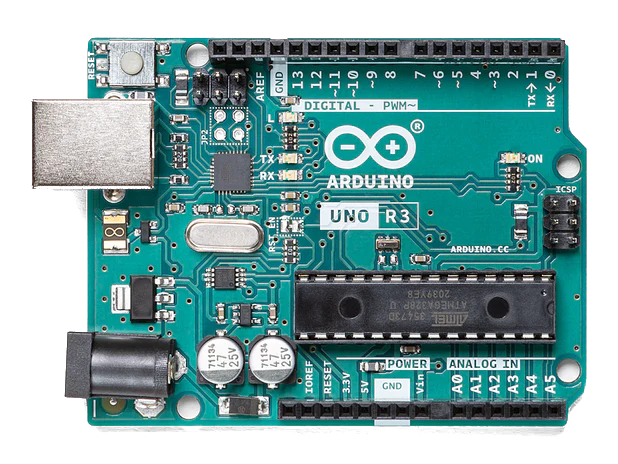
\includegraphics[width=0.6\textwidth]{arduino-uno.png}
		\caption{Arduino UNO\footnotemark}
	\end{figure}
}
\end{column}
\end{columns}
\footnotetext[1]{\url{https://www.raspberrypi.com/products/raspberry-pi-pico/}}
\footnotetext[2]{\url{https://store.arduino.cc/products/arduino-uno-rev3}}
\end{frame}

\begin{frame}{Integración X-Plane - Microcontrolador}
\large{Posibles aplicaciones}
\vspace{1cm}
\begin{itemize}
	\item <2-> Desarrollar sistemas de control
	\item <3-> Evaluar rendimiento de maniobras o en misiones
	\item <4-> Escribir código portable
\end{itemize}
\note<1>{
	Veamos brevemente algunas aplicaciones en que la comunicación entre los actores podría ser beneficiosa
}
\note<2>{
	Con la capacidad de analizar y responder al estado de la aeronave es posible desarrollar algoritmos de control o de piloto automático.
}
\note<3>{
	Gracias a que se trabaja con simulaciones, es posible manipular el estado arbitrariamente y ejecutar maniobras de manera iterativa reiniciándolas una y otra vez con fines de optimización
}
\note<4>{
	El código al correr en un microcontrolador será completamente portable y podrá ser reimplementado a cualquier otro sistema o aeronave real mientras se pueda acceder a una interfaz de datos.
}
\end{frame}

\subsection{Condiciones de diseño}
\begin{frame}{Condiciones de diseño}
El protocolo de comunicación establecido debe
\begin{itemize}
	\item <2-> Permitir acceso general a las variables internas de simulación.
	\item <3-> Funcionar en los microcontroladores más populares.
	\item <4-> Ser accesible para alumnos del departamento.
\end{itemize}
\end{frame}

\section{Establecimiento de protocolo}

\subsection{Soluciones existentes}
\begin{frame}[noframenumbering]
\subsectionpage
\end{frame}

\begin{frame}{MobiFlight}
	\begin{columns}
		\begin{column}{0.3\textwidth}{
			\begin{figure}[t]
				\centering
				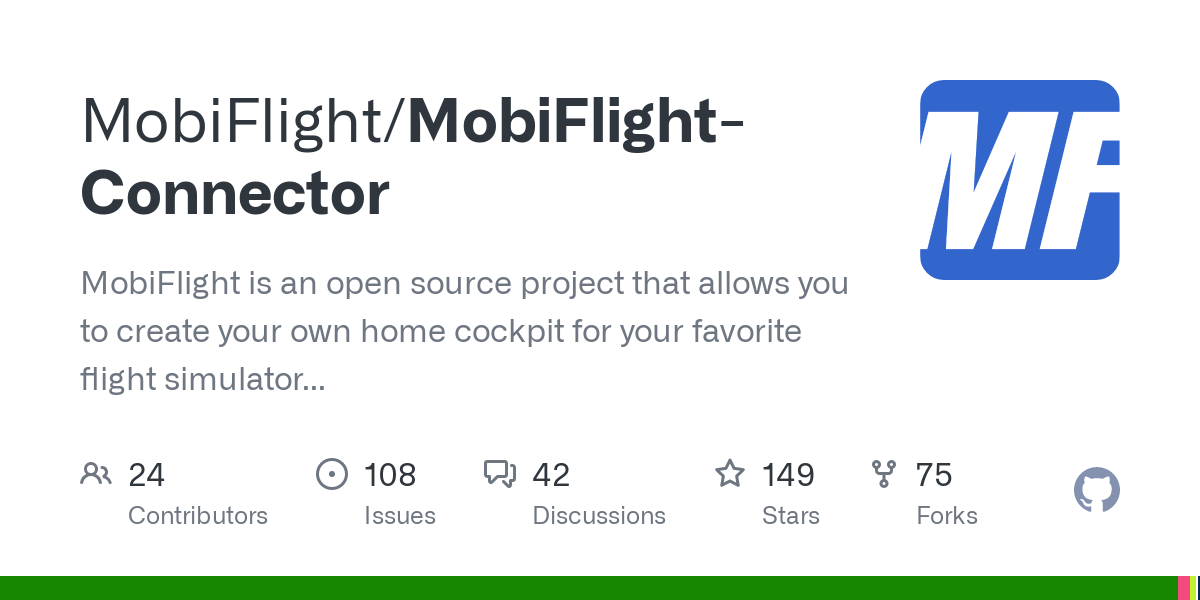
\includegraphics[width=\textwidth]{mobiflight_git.png}
				\footnotemark
			\end{figure}
		}
		\end{column}
		\begin{column}{0.69\textwidth}{
			\begin{figure}[t]
				\centering
				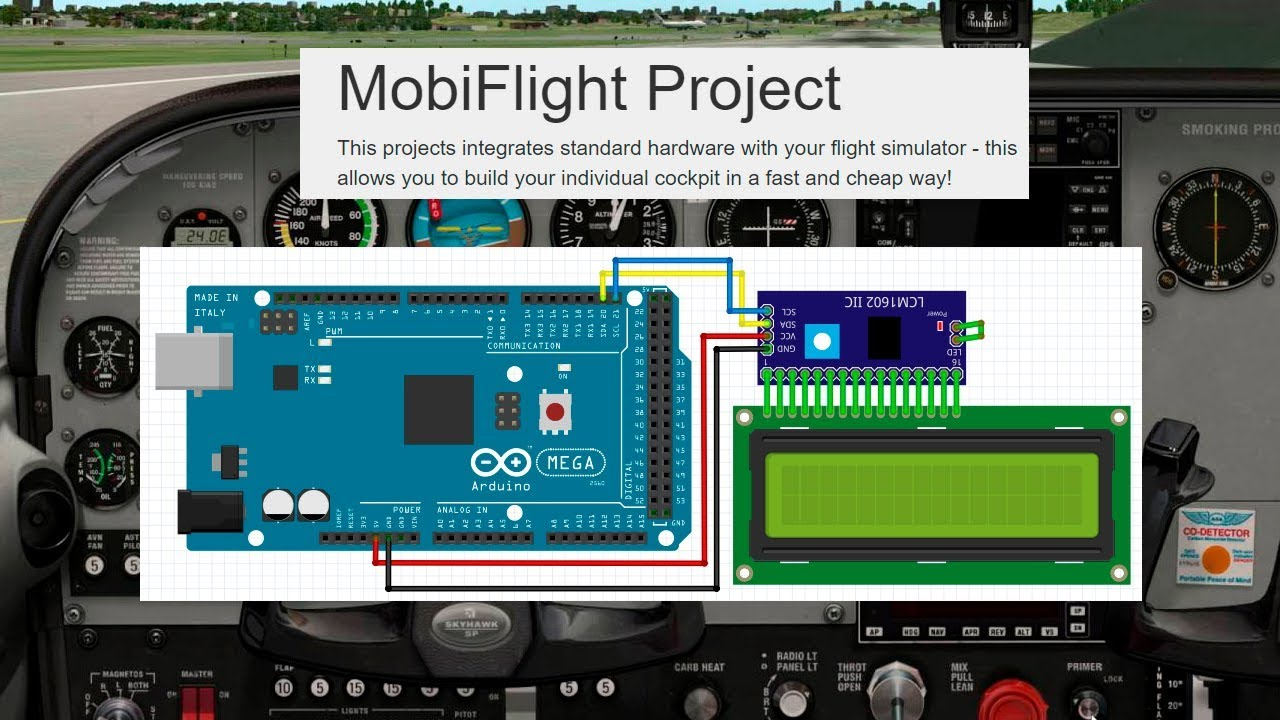
\includegraphics[width=\textwidth]{mobiflight.jpg}
				\footnotemark
			\end{figure}
		}
		\end{column}
	\end{columns}
	\footnotetext[1]{\url{https://github.com/MobiFlight/MobiFlight-Connector}}
	\footnotetext[2]{\href{https://www.youtube.com/watch?v=ja0tvTbaEnI}{Youtube - Mobiflight: Como usar un LCD Display / Using an LCD Display.}}
\end{frame}

\begin{frame}{SimVim}
	\begin{figure}[t]
		\centering
		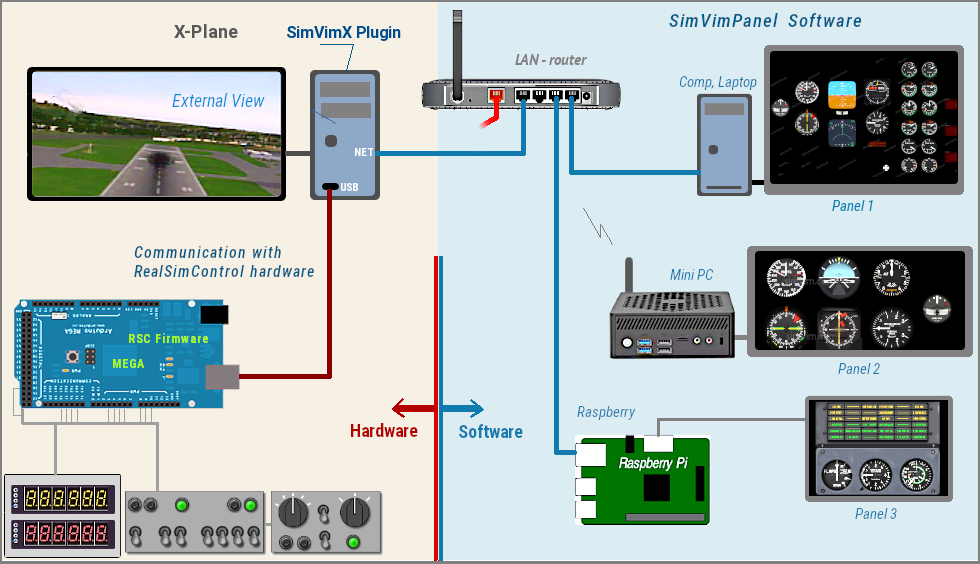
\includegraphics[width=0.8\textwidth]{simvim.png}
		\footnotemark
	\end{figure}
	\footnotetext{\url{https://simvim.com/}}
\end{frame}

\begin{frame}{\large Flight Simulator Universal Inter-Process Communication}
	\begin{figure}[t]
		\centering
		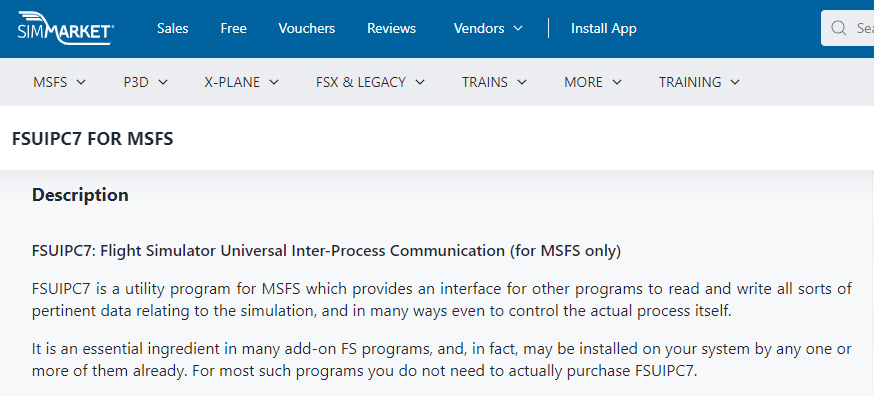
\includegraphics[width=0.9\textwidth]{fsuipc.png}
		\footnotemark
	\end{figure}
	\footnotetext{\url{https://secure.simmarket.com/john-dowson-fsuipc7-for-msfs.phtml}}
\end{frame}

\begin{frame}{NASA X-Plane Communications Toolbox}
	\begin{figure}[t]
		\centering
		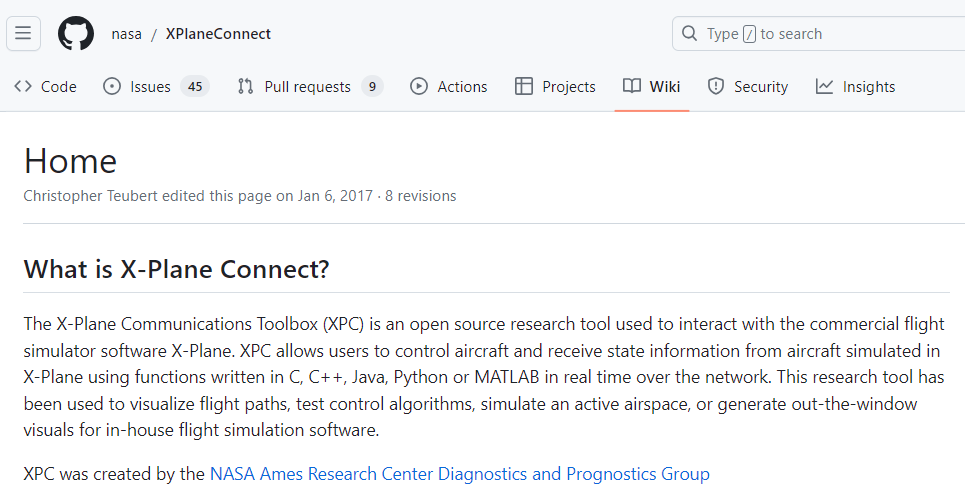
\includegraphics[width=0.9\textwidth]{nasa.png}
		\footnotemark
	\end{figure}
	\footnotetext{\url{https://github.com/nasa/XPlaneConnect/wiki}}
\end{frame}

\begin{frame}{Soluciones existentes}
Observaciones
\begin{itemize}
	\item <2-> MobiFlight y SimVim están diseñados para crear paneles de instrumentos con microcontroladores.
	\item <3-> FSUIPC y X-Plane Connect son de uso general, pero su documentación no contempla microcontroladores.
\end{itemize}
\visible<4-> {Conclusión}
\begin{itemize}
	\item <4-> Crear una nueva solución que cumpla las condiciones de diseño.
\end{itemize}
\end{frame}

%% Diseño del protocolo

\subsection{Diseño preliminar}
\begin{frame}[noframenumbering]
\subsectionpage
\end{frame}

\begin{frame}{Características de nueva solución}
\begin{itemize}
	\item <2-> Ser un programa intermediario entre el simulador y el microcontrolador.
	\item <3-> Interactuar con simulador por medio de FSUIPC.
	\item <4-> Extender FSUIPC con canales accesibles por microcontroladores.
\end{itemize}
\end{frame}

\begin{frame}{Diagrama}
	\foreach \n in {1,...,4}{
		\only<\n>{\fullsizegraphic{diagrama-fssp-step-\n.pdf}}
	}
\end{frame}	

\section{Implementación}
\begin{frame}[noframenumbering]
\sectionpage
\end{frame}

\begin{frame}{inoFS}
	\centering
	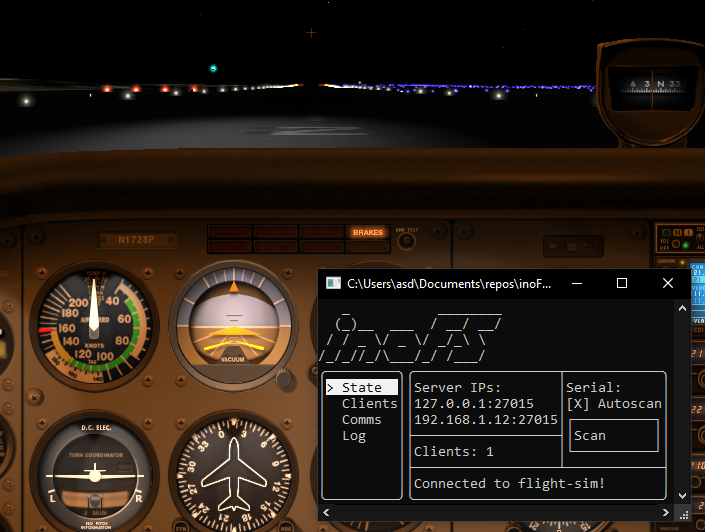
\includegraphics[width=0.6\textwidth]{inofs-1.PNG}
\end{frame}

\subsection{Características}

\begin{frame}{inoFS}
Características
\begin{itemize}
	\item <2-> Fácil instalación.
	\item <3-> Abre canales Serial y UDP por red local.
	\item <4-> Permite el acceso a variables internas del simulador por medio de FSUIPC.
	\item <5-> Interfaz gráfica sencilla para ayudar a identificar problemas.
\end{itemize}
\end{frame}

\begin{frame}{inoFS}
	\begin{columns}
	\begin{column}{0.45\textwidth}{
		\begin{figure}[t]
			\centering
			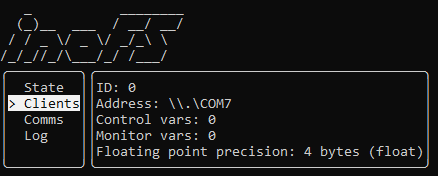
\includegraphics[width=1\textwidth]{inofs-clients.PNG}
			\caption{Pestaña Clientes}
	\end{figure}
	}
	\end{column}
	\begin{column}{0.45\textwidth}{
		\begin{figure}[t]
			\centering
			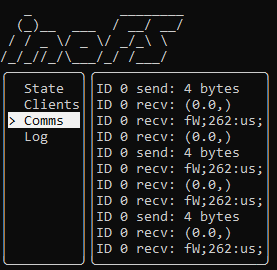
\includegraphics[width=0.8\textwidth]{inofs-comms.PNG}
			\caption{Pestaña Comunicaciones}
		\end{figure}
	}
	\end{column}
	\end{columns}
	\end{frame}

\begin{frame}{Protocolo}
\begin{itemize}
	\visible<2->{
		\item Mensajes estructurados
		\begin{itemize}
			\item Lectura
			\item Escritura
			\item Monitorear (Lectura continua)
			\item Controlar (Escritura continua)
		\end{itemize}
	}
	\visible<3->{
		\item Comandos enviados como cadenas de caracteres
		\item Datos enviados como bytes crudos
	}
\end{itemize}
\end{frame}

\begin{frame}[fragile]{Protocolo - Comando Escribir}
	\begin{lstlisting}[language=Python]
		# Header de mensaje
		header = bytes("inofs", "ascii")
		# Comando con variables a sobreescribir
		cmd = bytes("fW;310A:c;089A:s;", "ascii")
		# Variables
		input = 8
		throttle = (2/10) * 16384
		data = bytes(struct.pack("<ff", input, throttle), "ascii")
		# Evaluar largo del mensaje
		size = struct.pack("<i", len(cmd + data))
		# Empacar y enviar
		msg = header + size + cmd + data
		sys.stdout.buffer.write(msg)
	\end{lstlisting}
	Mensaje enviado por Serial\\
	\say{header} + \say{bytes del mensaje} + \say{comando} + \say{datos}
\end{frame}

\begin{frame}{Documentación}
\begin{itemize}
	\item Lista de variables de FSUIPC\\
	\url{https://www.projectmagenta.com/all-fsuipc-offsets/}
	\item Documentación inoFS en repositorio
	\url{https://github.com/qgerman2/inoFS}
\end{itemize}
	
	
\end{frame}

\section{Conclusión}
\begin{frame}[noframenumbering]
\sectionpage
\end{frame}

\begin{frame}{Conclusión}
\begin{itemize}
	\item<2-> Se establece el protocolo de comunicación de acuerdo a las condiciones de diseño.
	\item<3-> El programa es funcional, pero necesita más desarrollo.
	\item<4-> Con debida documentación, el programa podría ser utilizado por la comunidad.
\end{itemize}
\end{frame}

\begin{frame}[noframenumbering]
\centering
\Large \textbf{Gracias por su atención}
\end{frame}

\end{document}